\documentclass{beamer}


\usepackage[utf8]{inputenc}
\usepackage{pgfpages}
\usepackage{xcolor}

\setbeameroption{show notes}
\setbeameroption{show notes on second screen=left}

\usetheme{Warsaw}
\graphicspath{ {./images/}{../images/} }

\AtBeginSection[specialframe]
{
  \begin{frame}{Table of Contents}
   \tableofcontents[currentsection]
  \end{frame}
}

\title[Kcov - a single-step code coverage tool] %optional
{Kcov - a single-step code coverage tool}

%\subtitle{A short story}

\author{Simon Kågström}

\institute
{
  Net Insight\\
}

%\logo{\includegraphics[height=1.5cm]{lion-logo.png}}

\begin{document}

\begin{frame}
  \titlepage
  \note{My name is Simon Kågström and I work at Net Insight. Today I will present kcov, a code coverage collection and presentation tool. So let's get started!}
\end{frame}

\begin{frame}
  \frametitle{Motivation}
  \note<1->{
    \footnotesize
    I'll start with some motivation for the talk. Code coverage, as described by wikipedia, is the degree to which the source code of a program is executed when a particular test suite executes, measured in percentage.

    So let's say you're the developer of a particular piece of code, as shown on the slide. You run some tests on it, and collect code coverage to see how well your test suite actually works.
  }
  \note<2>{
    After code coverage collection, you will get a report which looks something like this. Red lines denote executable lines which have not been executed, green lines are executed lines. White lines is non-executable lines.

    Hmm... Hang on now, why is everything between line 128 and 143 marked as non-executable? Some of you might already have identified the code in question. This is the SSL/TLS bug known as ``goto fail''. Looking at line 127, you can see that the control flow will unconditionally jump to the fail label, so lines 128 to 143 are indeed unreachable.

    Stands out pretty clear from the coverage report don't you think? Modern compilers will also issue a warning on code like this.
    }
    
  \includegraphics<1>[height=8cm]{goto_fail_no_coverage}
  \includegraphics<2>[height=8cm]{goto_fail}
\end{frame}

\begin{frame}{Outline}
  \tableofcontents
  \note{This is the outline of the talk. I will start with a short discussion of problems and limitations with traditional tools, then introduce kcov and demonstrate some of the main features.

    I will then go into a bit of details about how kcov has been implemented, and give some lessons learned in the process.

  Finally, I will discuss some other features of kcov, which are perhaps a bit less relevant on a C++ workshop.}
\end{frame}

\section{Overview}
\subsection{Problems with traditional tools}
\begin{frame}[fragile]{Problems with traditional tools}
  \note{On UNIX, the traditional way of collecting code coverage has been to use gcov for collection, and lcov for HTML presentation, if desired. The process is a bit cumbersome, as can be seen in the example below. You first need a special --coverage option, which produces extra metadata files in the build directory. After running the program, you then get data for the actual execution in the build directory.

    After this, you need to run the presentation tool, like lcov, to get actual output. If the process crashes during execution, you will lose the coverage output altogether.

    % Mention clang

    Fortunately, using kcov does away with all these disadvantages, allowing collection without special compiler options, reporting without droppings and all done in a single step. Quite a sales pitch, don't you agree?}
  \begin{itemize}
  \item gcov + lcov is a multi-step process
  \item gcov leaves droppings after compilation/running
  \item A program which crashes will not generate coverage data
  \end{itemize}
  \begin{Example}
    \begin{semiverbatim}
     \scriptsize
\$ gcc -g -Wall --coverage goto-fail.c
\$ ./a.out
\$ ls
  a.out  goto-fail.c  goto-fail.gcda  goto-fail.gcno
\$ lcov --capture --directory project-dir --output-file coverage.info
\$ genhtml coverage.info --output-directory out
    \end{semiverbatim}
  \end{Example}
\end{frame}

\subsection{Kcov overview}
\begin{frame}{Kcov overview}
  \begin{itemize}
  \item Kcov started as a fork of Bcov by Thomas Neumann in 2010
  \item Bcov was a great idea, but I thought it could be improved upon
  \item It is not related to the kernel Kcov (and predates it by many years)
  \item<2-> Can you guess why it's called kcov?
  \end{itemize}

  \note{
    Kcov started as a fork of bcov, which doesn't rely on compile-time instrumentation of binaries, but instead uses the DWARF debug information present as long as you compile with -g. It can also produce lcov-like output.

    I thought bcov was a great idea, but it was still somewhat cumbersome to use, separating collection and reporting. The codebase was a bit difficult for me to follow, so I forked it instead of improving on the original project. Today I would problably not have done it that way.

    Guess the name! The original idea I had was to use kernel kprobes, which allows setting breakpoints on kernel code, while still retaining the userspace functionality. K therfore stands for kernel.
  }
\end{frame}

\subsection{Main features of kcov}
\begin{frame}{Interactive Demo!}
  \note{
      \begin{itemize}
      \item Demo: Make sure /tmp/kcov is empty

      \item kcov /tmp/kcov projects/build/kcov/target/src/kcov

      \item Show result in browser

      \item Show how a single file looks, describe 1/3 etc

      \item Show file list again, note /usr/include etc

      \item Remove /tmp/kcov. All output is placed in the out-directory, so this cleans up everything from the coverage run

      \item Run again with --include-pattern

      \item Run calc, show merged report

      \item Run kcov with --include-pattern, note that --exclude-pattern and paths also exist

      \item Run kcov on another program (calc?), show that output is merged
    \end{itemize}
  }
\end{frame}

\subsection{Integration with CI systems}
\begin{frame}{Integration with CI systems}
  \note{Kcov also integrates with several systems and sites for continous integration. Jenkins has a plugin for Cobertura, normally a Java code coverage collection tool. As kcov produces XML output for Cobertura, it's easy to integrate in that environment. SonarQube is handled in a similar way.

 It also supports some popular cloud services. NEXT. It can upload directly to coveralls, which is often used together with travis-ci. Coveralls is an easy way to get fancy web stats for your project coverage. NEXT. Similarly, codecov.io is also easy to integrate, but supports kcov directly from the upstream project.

Personally, I haven't picked a favourite cloud coverage service just yet, but instead use both with travis-ci and added dual badges on github.
  }
  \begin{itemize}
  \item Jenkins and SonarQube output is generated by kcov
  \item \textcolor<2>{red}{Uploading to Coveralls.io is built-in}
  \item \textcolor<3>{red}{Uploading to Codecov.io is supported by the upstream project}
  \end{itemize}
  \includegraphics<1-2>[height=6cm]{coveralls}
  \includegraphics<3>[height=6cm]{codecov}
\end{frame}

\section{How kcov works}
\begin{frame}{Design}
  \note{}
  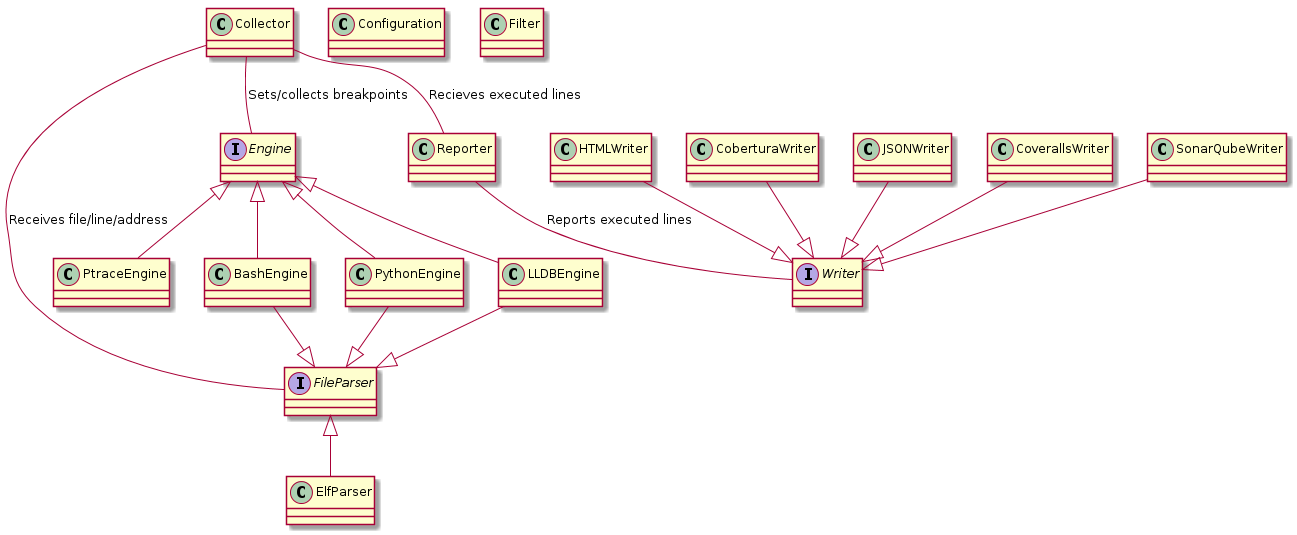
\includegraphics[width=\linewidth]{design}
\end{frame}

\subsection{Elves, dwarves and breakpoints}
\begin{frame}[fragile]{Dwarf stabs Elf}
  \note{The world of binary file formats and debug information is full of funny names. Stabs is an older format for debug information, but ELF, Mach-O and Dwarf is in active use on Unix systems.

    Kcov relies on Dwarf debug information to set a breakpoint on each executable line in the program. The debug information contains records of file:line to address mappings, which is exactly what kcov needs. NEXT. In the disassembly output, you can see this as the addresses marked in red here, which correspond to DWARF entries.
% Disassembly here
    
    Kcov executes the program in stopped state via ptrace, sets all breakpoints and then lets the program continue again. On each executed breakpoint, kcov marks the file:line pair as executed, removes the breakpoint and lets the program continue again. That's the basic way kcov works.
  }
  \begin{itemize}
    \item \textbf{elf\_version} must be called at program start!
  \end{itemize}
  \begin{Example}
    \begin{semiverbatim}
      \scriptsize
 124:     return (void*)op\_create(RPAR);
\textcolor<2>{red}{400ff7}:       bf 30 00 00 00          mov    \$0x30,\%edi
400ffc:       e8 1f 05 00 00          callq  401520 <op\_create>
401001:       e9 20 ff ff ff          jmpq   400f26 <ts\_next\_token+0x46>
401006:       66 2e 0f 1f 84 00 00    nopw   \%cs:0x0(\%rax,\%rax,1)
40100d:       00 00 00
 125: p\_state->last\_token\_is\_od = 0;
\textcolor<2>{red}{401010}:       c7 43 08 00 00 00 00    movl   \$0x0,0x8(\%rbx)
 126: return (void*)op\_create(op);
\textcolor<2>{red}{401017}:       bf 04 00 00 00          mov    \$0x4,\%edi
40101c:       e8 ff 04 00 00          callq  401520 <op\_create>
   \end{semiverbatim}
   \end{Example}
 % Disassembly
  % file:line -> addr
  % Cleared once it has been executed
\end{frame}

\subsection{Implementation quirks on different architectures}
\begin{frame}{kcov on Linux, FreeBSD and Mac OSX}
  \note{There is no fully standardized way of setting and controlling breakpoints on UNIX.The ancient ptrace is typically used for this, through PEEKTEXT/POKETEXT options. The original bcov implementation is the base for the Linux implementation, but Alan Somers have more recently extracted the OS-dependent parts and ported Kcov to FreeBSD.

OSX works in an entirently different way though. The key difference between OSX and Linux/FreeBSD is that OSX uses it's own binary format, Mach-O. So we now have Dwarves, Elves and Mach-O. For ELF, we have libelf to do the parsing, but Apple doesn't publish a library for Mach-O. I therefore opted on a simpler solution on OSX. The LLDB debugger comes with the development environment on OSX, and it conveniently offers a nice C++ API.

So on OSX, the entire parsing, process control and breakpoint setting is only 486 lines of code. The disadvantage with the LLDB implementation is that it's significantly slower than using regular ptrace. During normal debugging, you typically don't set tens of thousands of breakpoints!
  }
\end{frame}

\subsection{ELF/Dwarf implementation quirks}
\begin{frame}{Libelf}
  % file:line maps to an invalid address
  % ptrace: Does not set breakpoints, modifies memory
  % ptrace is not recursive, can't strace kcov
  % When a process stops, you need to dump the register file and find the PC. This is
  % architecture and OS dependent
\end{frame}

\section{Other kcov features}

\subsection{Python/Bash}
\begin{frame}{Python}
\end{frame}

\subsection{System mode}
\begin{frame}{System mode}
\end{frame}

\end{document}

%Kcov - a single-step code coverage tool

%- Motivation

%  - What is code coverage?

%  - goto fail

% - Outline of the presentation


% - Setting: UNIX


% - Problems with gcov + lcov etc

%  - Multiple steps

%  - Loses data on program crash


%- Basic demo of kcov

%  - Explain how the output looks, 1/2 etc

%- History

%  - Bcov by Thomas Neumann

%  - Kernel kcov - not related

%- Some features

%  - What I use if for

%  - Demo with filtering, merging etc


%- How kcov works

%  - A bit about how gcov works

%  - Breakpoints

%  - Differences between OSX and Linux/FreeBSD

 % - Complain a bit about elf_version/libdwarf etc.


% - What about speed?
